\newcommand{\TRESicmin}{1.85\xspace}
\newcommand{\TRESicmax}{3.10\xspace}
\newcommand{\TRESicNoveNoveMin}{1.62\xspace}
\newcommand{\TRESicNoveNoveMax}{3.33\xspace}
\newcommand{\TRESnZero}{26\xspace}


Foram retiradas 200 amostras, sem reposição, com tamanhos $n$ = 4, 8, 16, 30 e 100, 
dentre os 4986 alunos que possuíam um valor definido para a variável \textit{Renda}.
A população possuí média $\mu$ = ${\UMx}$ para a variável \textit{Renda}, com desvio padrão $\sigma$ = ${\UMsd}$.
A \autoref{tab:q1} apresentam os valores da média e desvio padrão para cada tamanho
de amostra e seu respectivo valor esperado de desvio padrão ($\frac{\sigma}{\sqrt{n}}$).

\begin{table}[h]
\centering
\caption{Valores da média e desvio padrão das médias amostrais da variável \textit{Renda}.}
\label{tab:q1}
\vspace{0.5em}
\begin{tabular}{l r r r}
	\toprule
	\textbf{\specialcell{c}{Tamanho da\\Amostra}} & \textbf{Média} & \textbf{\specialcell{c}{Desvio\\Padrão}} & \textbf{$\frac{\sigma}{\sqrt{n}}$}\\
	\midrule
	$4$       & ${\UMxQuatro}$   & ${\UMsdQuatro}$   & ${\UMsdeQuatro}$   \\
	$8$       & ${\UMxOito}$   & ${\UMsdOito}$   & ${\UMsdeOito}$   \\
	$16$      & ${\UMxDezesseis}$  & ${\UMsdDezesseis}$  & ${\UMsdeDezesseis}$  \\
	$30$      & ${\UMxTrinta}$  & ${\UMsdTrinta}$  & ${\UMsdeTrinta}$  \\
	$100$     & ${\UMxCem}$ & ${\UMsdCem}$ & ${\UMsdeCem}$ \\
	\bottomrule
\end{tabular}
\end{table}

\subsection{Valor esperado da média amostral}
Na \autoref{tab:q1} é possível observar que a medida que se aumenta o tamanho da amostra o valor da média amostral fica cada vez mais próximo do valor da média populacional, que é de ${\UMx}$.


\subsection{Valor esperado do desvio padrão da média amostral}
Conforme indicado na \autoref{tab:q1}, os valores de desvio padrão das amostras ficam mais próximos dos valores de $\frac{\sigma}{\sqrt{n}}$ à medida que se aumenta o tamanho das amostras.

\subsection{Distribuição amostral da média}
Conforme indicado na Figura \ref{fig:distribuicao-amostral}, à medida que se aumenta o tamanho das amostras
a distribuição amostral da média se torna similar à uma distribuição normal.

\begin{figure}
	\centering
	\begin{subfigure}[b]{0.48\textwidth}
		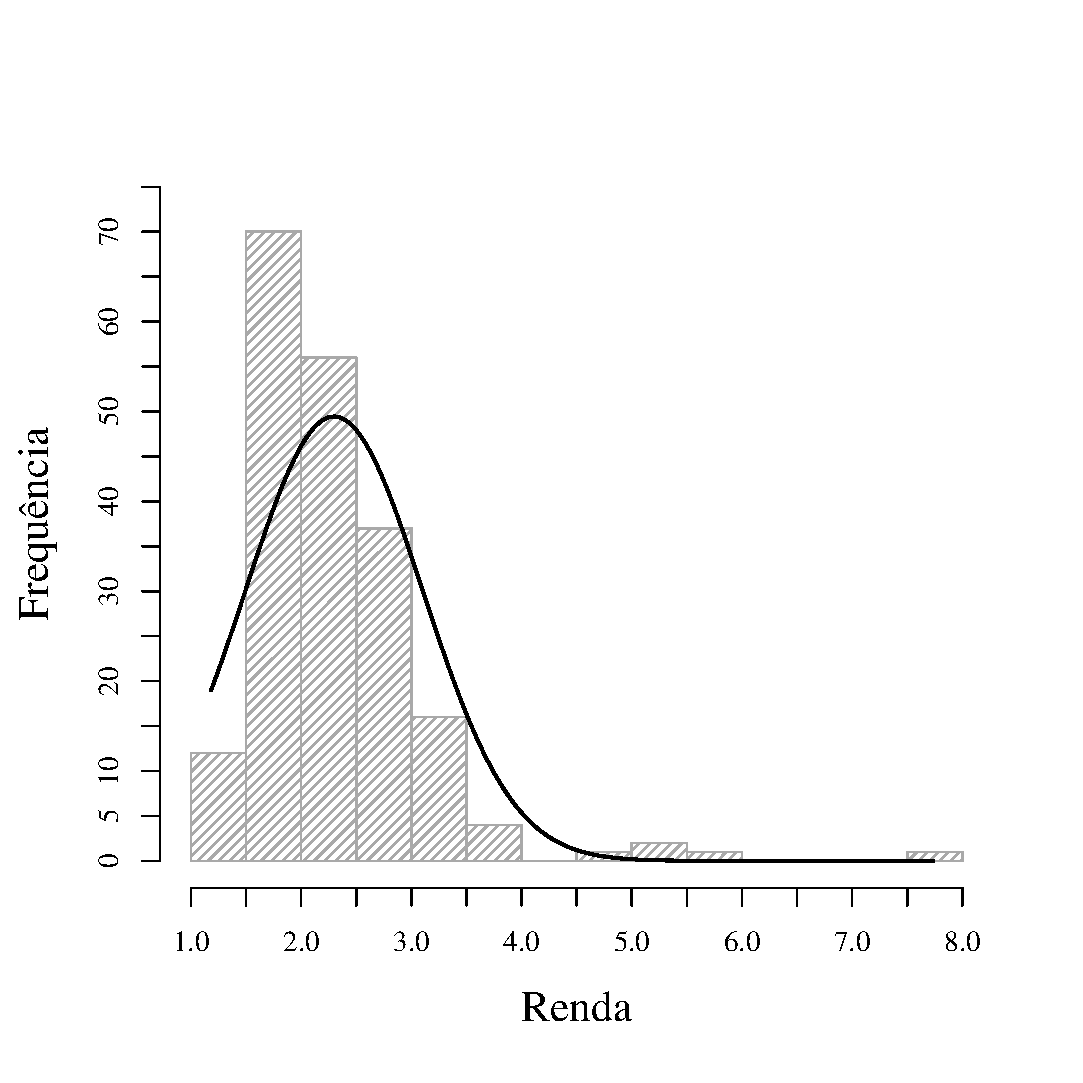
\includegraphics[width=\textwidth]{plots/histogram_renda_n4.eps}
		\caption{}
		\label{fig:m4}
	\end{subfigure}
	~
	\begin{subfigure}[b]{0.48\textwidth}
		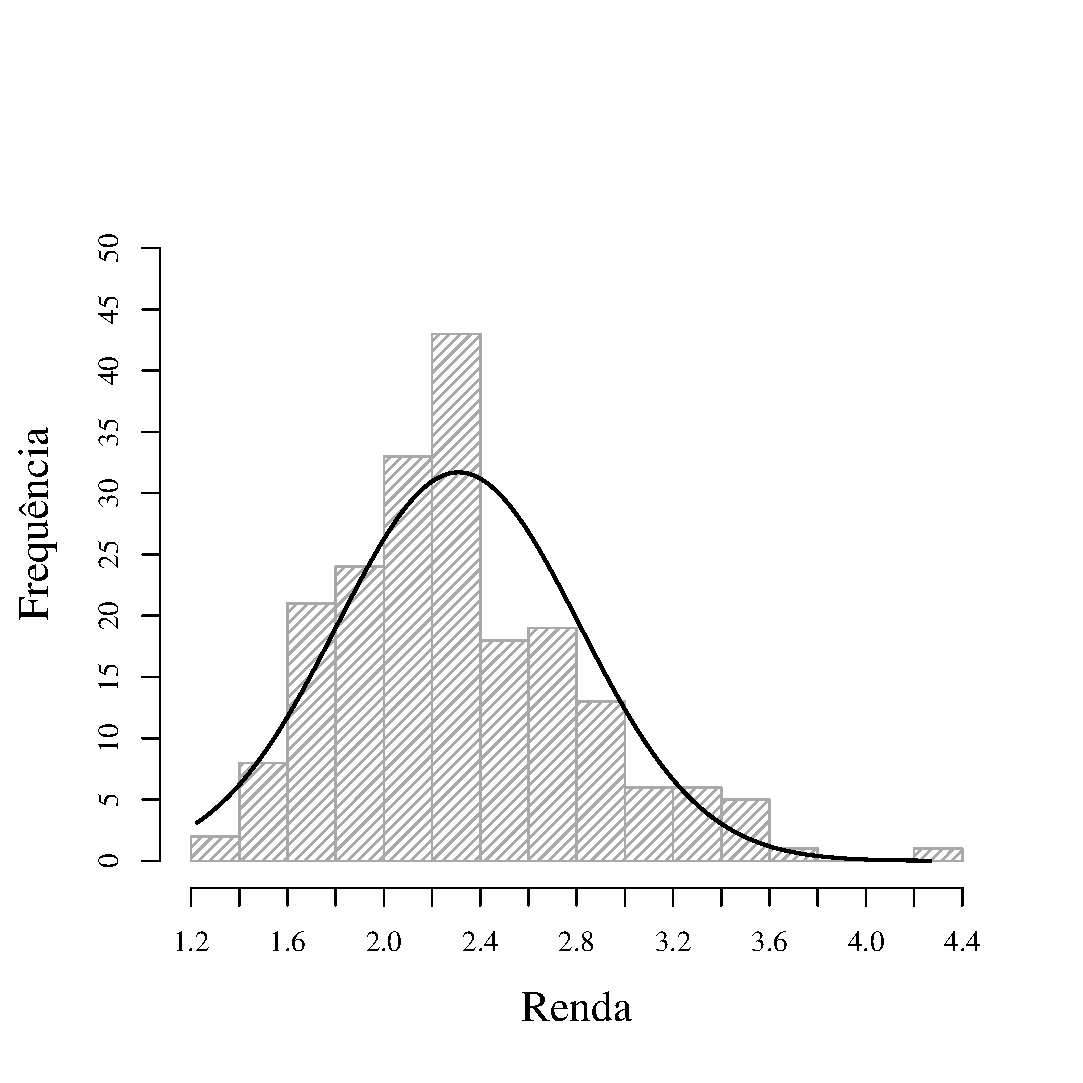
\includegraphics[width=\textwidth]{plots/histogram_renda_n8.eps}
		\caption{}
		\label{fig:m8}
	\end{subfigure}
	\\
	\begin{subfigure}[b]{0.48\textwidth}
		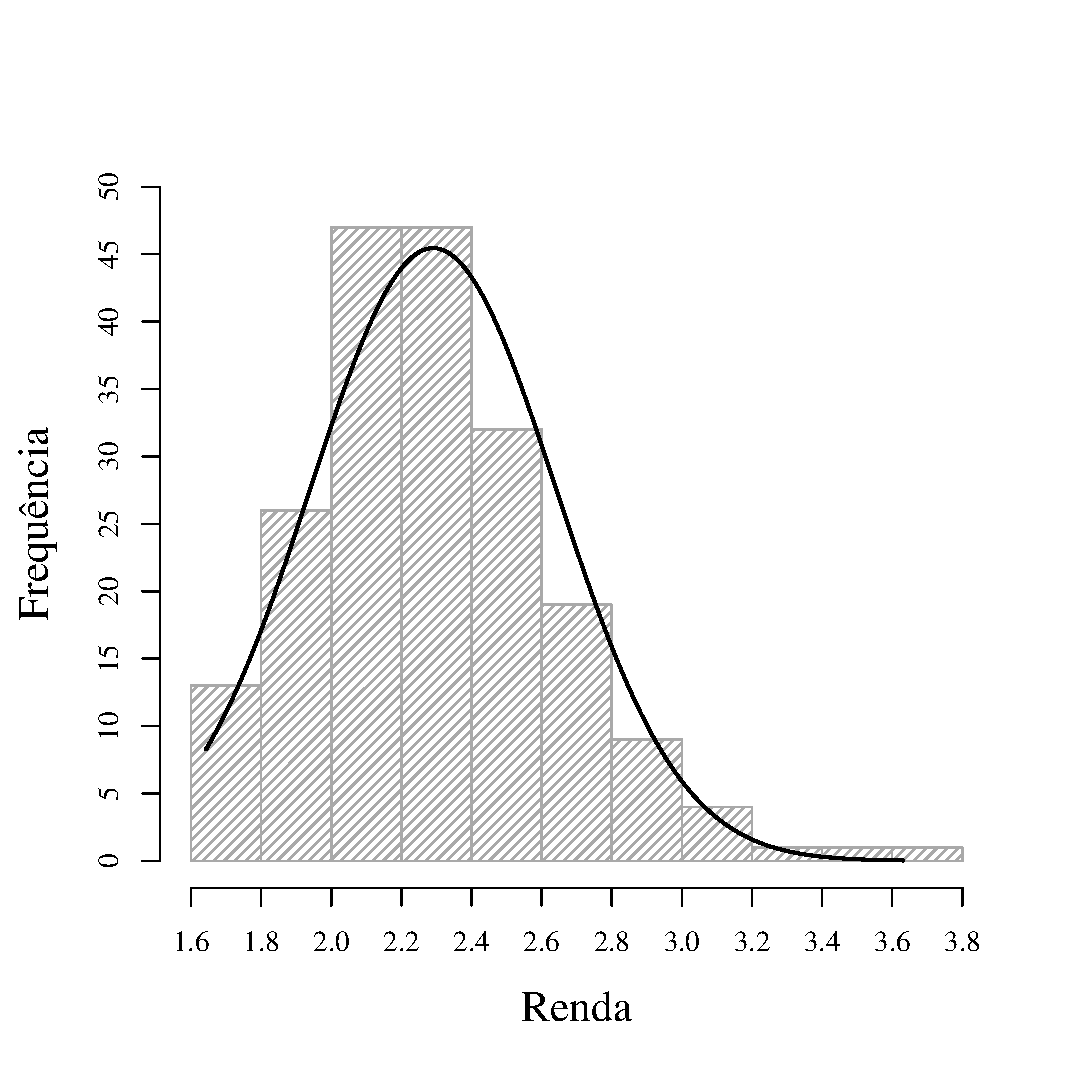
\includegraphics[width=\textwidth]{plots/histogram_renda_n16.eps}
		\caption{}
		\label{fig:m16}
	\end{subfigure}
	~
	\begin{subfigure}[b]{0.48\textwidth}
		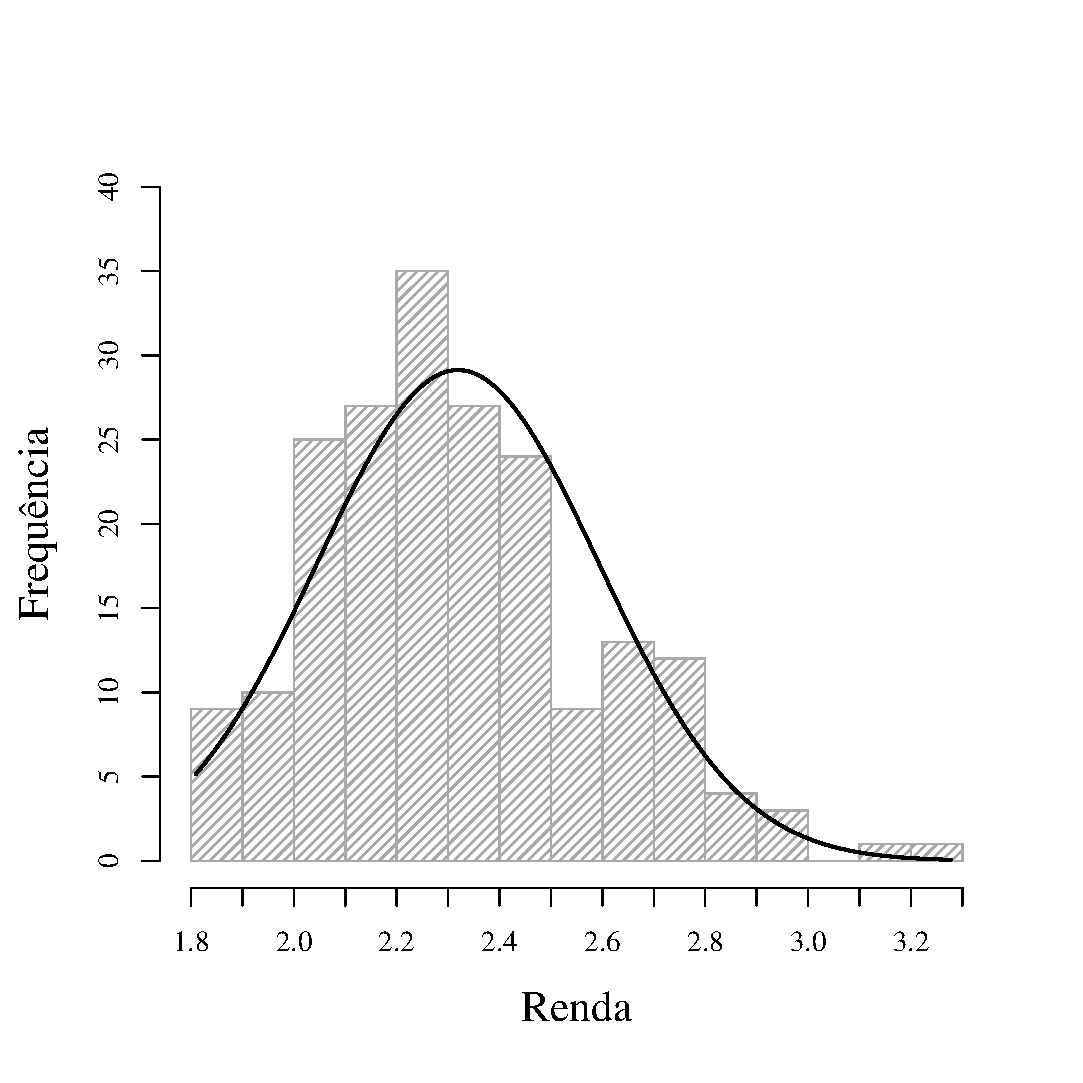
\includegraphics[width=\textwidth]{plots/histogram_renda_n30.eps}
		\caption{}
		\label{fig:m30}
	\end{subfigure}
	\\
	\begin{subfigure}[b]{0.48\textwidth}
		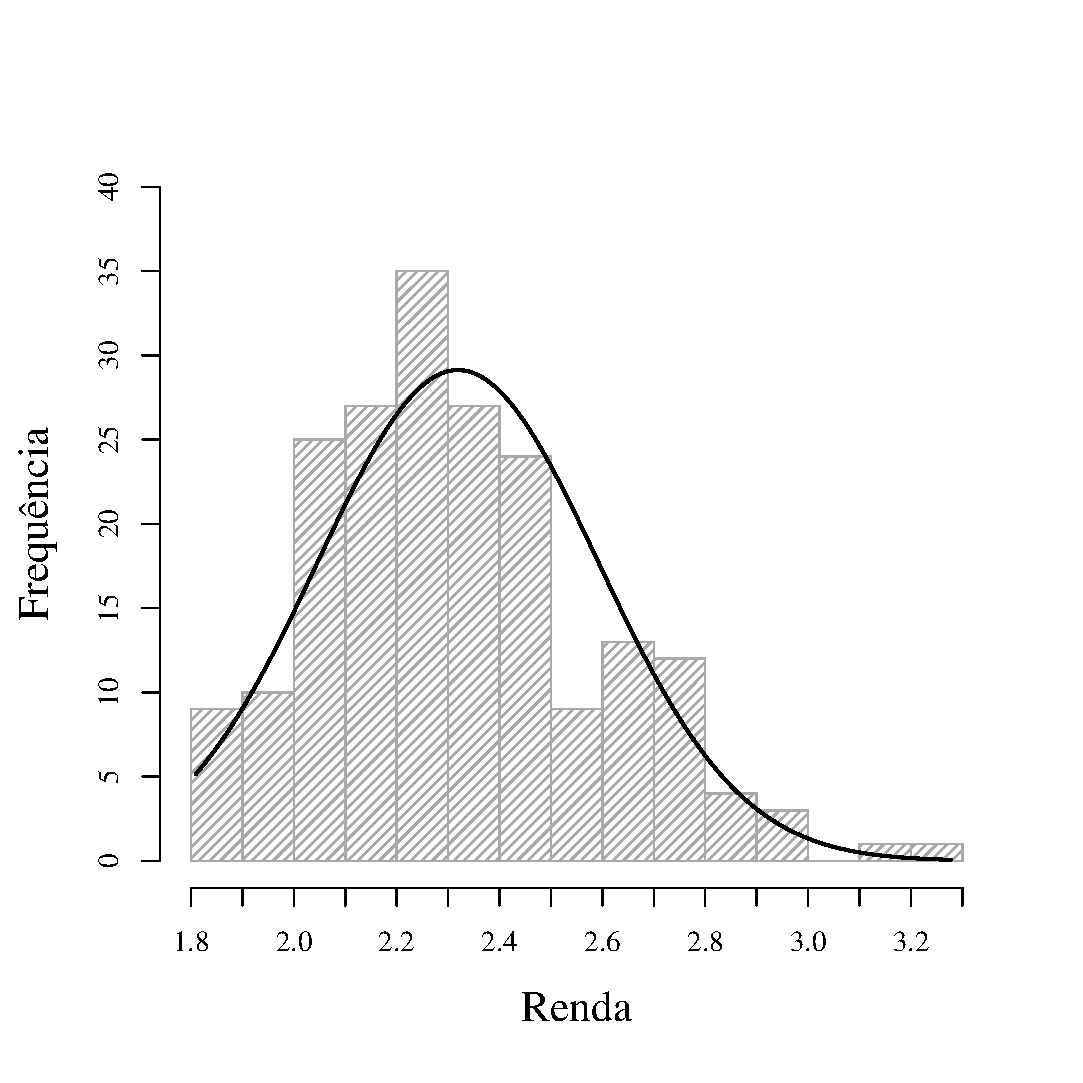
\includegraphics[width=\textwidth]{plots/histogram_renda_n30.eps}
		\caption{}
		\label{fig:m30}
	\end{subfigure}
	\label{fig:distribuicao-amostral}
	\caption{Distribuições amostrais das médias para amostras de tamanho 4(a), 8(b), 16(c), 30(d) e 100(e).}
\end{figure}

\FloatBarrier
